%%%%%%%%%%%%%%%%%%%%%%%%%%%%%%%%%%%%%%%%%
% Programming/Coding Assignment
% LaTeX Template
%
% This template has been downloaded from:
% http://www.latextemplates.com
%
% Original author:
% Ted Pavlic (http://www.tedpavlic.com)
%
% Note:
% The \lipsum[#] commands throughout this template generate dummy text
% to fill the template out. These commands should all be removed when 
% writing assignment content.
%
% This template uses a Perl script as an example snippet of code, most other
% languages are also usable. Configure them in the "CODE INCLUSION 
% CONFIGURATION" section.
%
%%%%%%%%%%%%%%%%%%%%%%%%%%%%%%%%%%%%%%%%%

%----------------------------------------------------------------------------------------
%	PACKAGES AND OTHER DOCUMENT CONFIGURATIONS
%----------------------------------------------------------------------------------------

\documentclass{article}

\usepackage{fancyhdr} % Required for custom headers
\usepackage{lastpage} % Required to determine the last page for the footer
\usepackage{extramarks} % Required for headers and footers
\usepackage[usenames,dvipsnames]{color} % Required for custom colors
\usepackage{graphicx} % Required to insert images
\usepackage{listings} % Required for insertion of code
\usepackage{courier} % Required for the courier font
\usepackage{lipsum} % Used for inserting dummy 'Lorem ipsum' text into the template

% Margins
\topmargin=-0.45in
\evensidemargin=0in
\oddsidemargin=0in
\textwidth=6.5in
\textheight=9.0in
\headsep=0.25in

\linespread{1.1} % Line spacing

% Set up the header and footer
\pagestyle{fancy}
\lhead{\hmwkAuthorName} % Top left header
\chead{\hmwkClass\ (\hmwkClassInstructor\ \hmwkClassTime): \hmwkTitle} % Top center head
\rhead{\firstxmark} % Top right header
\lfoot{\lastxmark} % Bottom left footer
\cfoot{} % Bottom center footer
\rfoot{Page\ \thepage\ of\ \protect\pageref{LastPage}} % Bottom right footer
\renewcommand\headrulewidth{0.4pt} % Size of the header rule
\renewcommand\footrulewidth{0.4pt} % Size of the footer rule

\setlength\parindent{0pt} % Removes all indentation from paragraphs

%----------------------------------------------------------------------------------------
%	CODE INCLUSION CONFIGURATION
%----------------------------------------------------------------------------------------

\definecolor{MyDarkGreen}{rgb}{0.0,0.4,0.0} % This is the color used for comments
\lstloadlanguages{Perl} % Load Perl syntax for listings, for a list of other languages supported see: ftp://ftp.tex.ac.uk/tex-archive/macros/latex/contrib/listings/listings.pdf
\lstset{language=Perl, % Use Perl in this example
        frame=single, % Single frame around code
        basicstyle=\small\ttfamily, % Use small true type font
        keywordstyle=[1]\color{Blue}\bf, % Perl functions bold and blue
        keywordstyle=[2]\color{Purple}, % Perl function arguments purple
        keywordstyle=[3]\color{Blue}\underbar, % Custom functions underlined and blue
        identifierstyle=, % Nothing special about identifiers                                         
        commentstyle=\usefont{T1}{pcr}{m}{sl}\color{MyDarkGreen}\small, % Comments small dark green courier font
        stringstyle=\color{Purple}, % Strings are purple
        showstringspaces=false, % Don't put marks in string spaces
        tabsize=5, % 5 spaces per tab
        %
        % Put standard Perl functions not included in the default language here
        morekeywords={rand},
        %
        % Put Perl function parameters here
        morekeywords=[2]{on, off, interp},
        %
        % Put user defined functions here
        morekeywords=[3]{test},
       	%
        morecomment=[l][\color{Blue}]{...}, % Line continuation (...) like blue comment
        numbers=left, % Line numbers on left
        firstnumber=1, % Line numbers start with line 1
        numberstyle=\tiny\color{Blue}, % Line numbers are blue and small
        stepnumber=5 % Line numbers go in steps of 5
}

% Creates a new command to include a perl script, the first parameter is the filename of the script (without .pl), the second parameter is the caption
\newcommand{\perlscript}[2]{
\begin{itemize}
\item[]\lstinputlisting[caption=#2,label=#1]{#1.pl}
\end{itemize}
}

%----------------------------------------------------------------------------------------
%	DOCUMENT STRUCTURE COMMANDS
%	Skip this unless you know what you're doing
%----------------------------------------------------------------------------------------

% Header and footer for when a page split occurs within a problem environment
\newcommand{\enterProblemHeader}[1]{
\nobreak\extramarks{#1}{#1 continued on next page\ldots}\nobreak
\nobreak\extramarks{#1 (continued)}{#1 continued on next page\ldots}\nobreak
}

% Header and footer for when a page split occurs between problem environments
\newcommand{\exitProblemHeader}[1]{
\nobreak\extramarks{#1 (continued)}{#1 continued on next page\ldots}\nobreak
\nobreak\extramarks{#1}{}\nobreak
}

\setcounter{secnumdepth}{0} % Removes default section numbers
\newcounter{homeworkProblemCounter} % Creates a counter to keep track of the number of problems

\newcommand{\homeworkProblemName}{}
\newenvironment{homeworkProblem}[1][Problem \arabic{homeworkProblemCounter}]{ % Makes a new environment called homeworkProblem which takes 1 argument (custom name) but the default is "Problem #"
\stepcounter{homeworkProblemCounter} % Increase counter for number of problems
\renewcommand{\homeworkProblemName}{#1} % Assign \homeworkProblemName the name of the problem
\section{\homeworkProblemName} % Make a section in the document with the custom problem count
\enterProblemHeader{\homeworkProblemName} % Header and footer within the environment
}{
\exitProblemHeader{\homeworkProblemName} % Header and footer after the environment
}

\newcommand{\problemAnswer}[1]{ % Defines the problem answer command with the content as the only argument
\noindent\framebox[\columnwidth][c]{\begin{minipage}{0.98\columnwidth}#1\end{minipage}} % Makes the box around the problem answer and puts the content inside
}

\newcommand{\homeworkSectionName}{}
\newenvironment{homeworkSection}[1]{ % New environment for sections within homework problems, takes 1 argument - the name of the section
\renewcommand{\homeworkSectionName}{#1} % Assign \homeworkSectionName to the name of the section from the environment argument
\subsection{\homeworkSectionName} % Make a subsection with the custom name of the subsection
\enterProblemHeader{\homeworkProblemName\ [\homeworkSectionName]} % Header and footer within the environment
}{
\enterProblemHeader{\homeworkProblemName} % Header and footer after the environment
}

%----------------------------------------------------------------------------------------
%	NAME AND CLASS SECTION
%----------------------------------------------------------------------------------------

\newcommand{\hmwkTitle}{FE-Assignment\ \#02} % Assignment title
\newcommand{\hmwkDueDate}{Friday,\ January\ 29,\ 2016} % Due date
\newcommand{\hmwkClass}{MA\ 374} % Course/class
\newcommand{\hmwkClassTime}{} % Class/lecture time
\newcommand{\hmwkClassInstructor}{} % Teacher/lecturer
\newcommand{\hmwkAuthorName}{Silvi Pandey (130123045)} % Your name

%----------------------------------------------------------------------------------------
%	TITLE PAGE
%----------------------------------------------------------------------------------------

\title{
\vspace{2in}
\textmd{\textbf{\hmwkClass:\ \hmwkTitle}}\\
\normalsize\vspace{0.1in}\small{Due\ on\ \hmwkDueDate}\\
\vspace{0.1in}\large{\textit{\hmwkClassInstructor\ \hmwkClassTime}}
\vspace{3in}
}

\author{\textbf{\hmwkAuthorName}}
\date{} % Insert date here if you want it to appear below your name

%----------------------------------------------------------------------------------------

\begin{document}

\maketitle

%----------------------------------------------------------------------------------------
%	TABLE OF CONTENTS
%----------------------------------------------------------------------------------------

%\setcounter{tocdepth}{1} % Uncomment this line if you don't want subsections listed in the ToC

\newpage

%----------------------------------------------------------------------------------------
%	PROBLEM 1
%----------------------------------------------------------------------------------------

% To have just one problem per page, simply put a \clearpage after each problem
\begin{center}
\textbf{PROBLEM 1}
\end{center}

Write a program to determine the initial price of an European call and an European put option in the binomial
model with the following data :
$$S(0) = 100 \quad K = 100 \quad T = 1 \quad M = 100 \quad r = 8\% \quad \sigma = 20\%$$
Use the following two sets of u and d for your program.\\
(a) Set 1 : $u = e^{\sigma \sqrt{\Delta t}}$ , $d = e^{-\sigma \sqrt{\Delta t}}$\\
(b) Set 2 : $u = e^{\sigma \sqrt{\Delta t} + (r-\frac{1}{2}\sigma ^{2})\Delta t}$ , $d = e^{-\sigma \sqrt{\Delta t} + (r-\frac{1}{2}\sigma ^{2})\Delta t}$

Here $\Delta t = \frac{T}{M}$ with M being the number of subintervals in the time interval [0,T]. Use the continuous
compounding convention in your calculations (i.e., both in \~p and in the pricing formula).\\
Now, plot the initial prices of both call and put options (for both the above sets of u and d) by varying one of the
parameters at a time (as given below) while keeping the other parameters fixed (as given above) :\\
(a) S(0).\\
(b) K.\\
(c) r.\\
(d) $\sigma$\\
(e) M (Do this for three values of K, K = 95 , 100 , 105).

\begin{center}
\textbf{SOLUTION}
\end{center}

\textbf{European Call Option }\\
In the following plots, the left plot is for Set - 1 (u,d) and the right one corresponds to Set - 2.\\
(a) Varying S(0) :\\
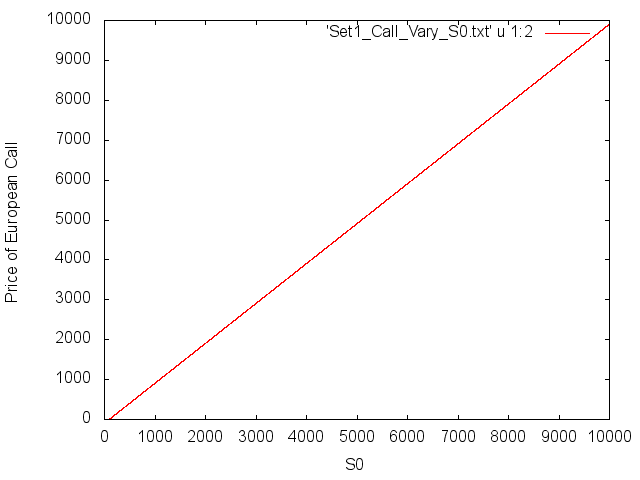
\includegraphics[width =80mm]{Set1_Call_Vary_S0}
\quad \quad
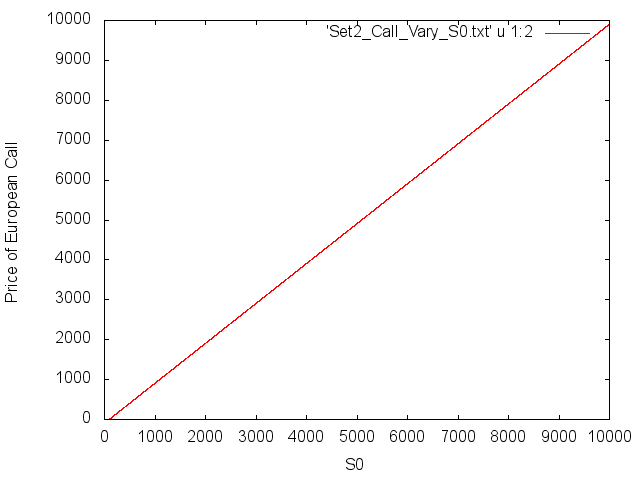
\includegraphics[width =80mm]{Set2_Call_Vary_S0}\\
(b) Varying K :\\
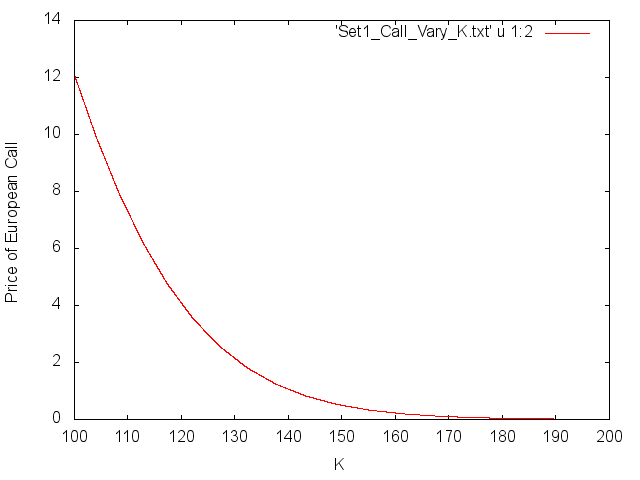
\includegraphics[width =80mm]{Set1_Call_Vary_K}
\quad \quad
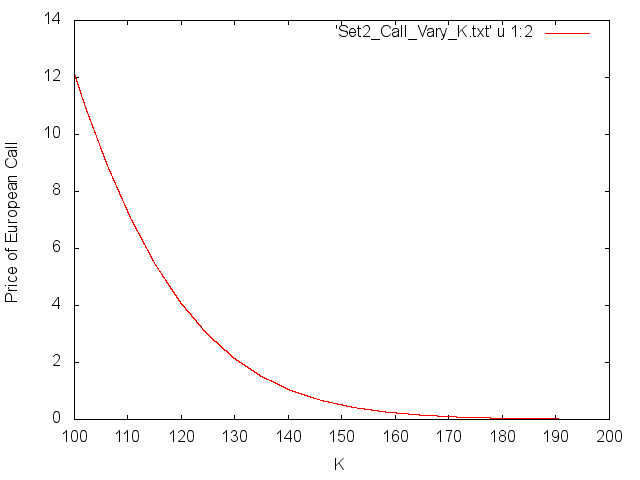
\includegraphics[width =80mm]{Set2_Call_Vary_K}\\
(c) Varying r :\\
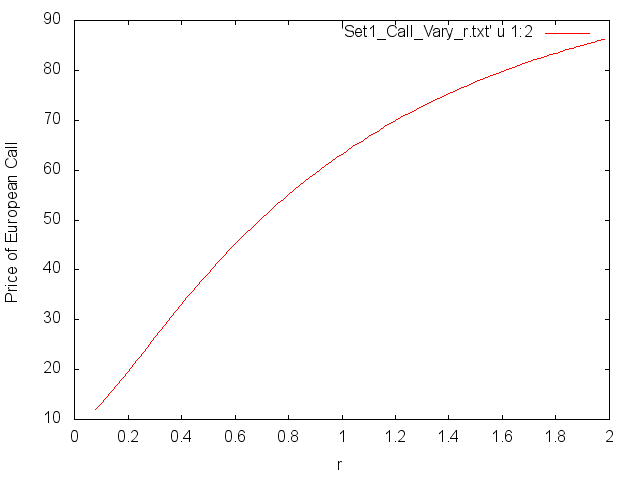
\includegraphics[width =80mm]{Set1_Call_Vary_r}
\quad \quad
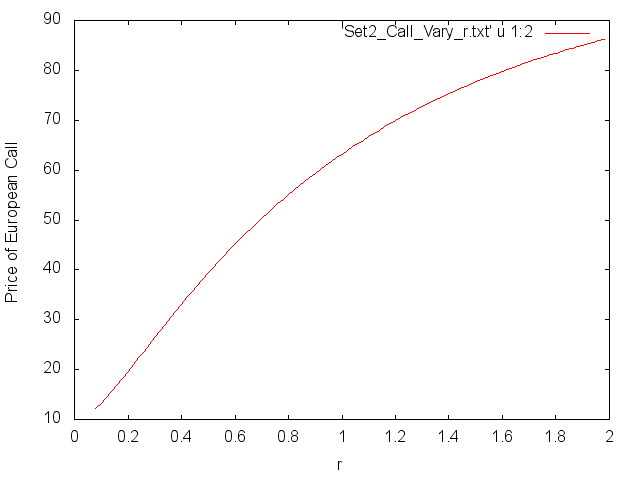
\includegraphics[width =80mm]{Set2_Call_Vary_r}\\
(d) Varying $\sigma$ :\\
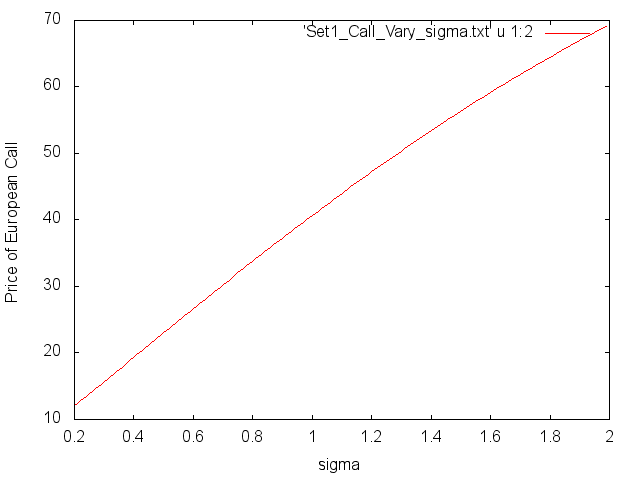
\includegraphics[width =80mm]{Set1_Call_Vary_sigma}
\quad \quad
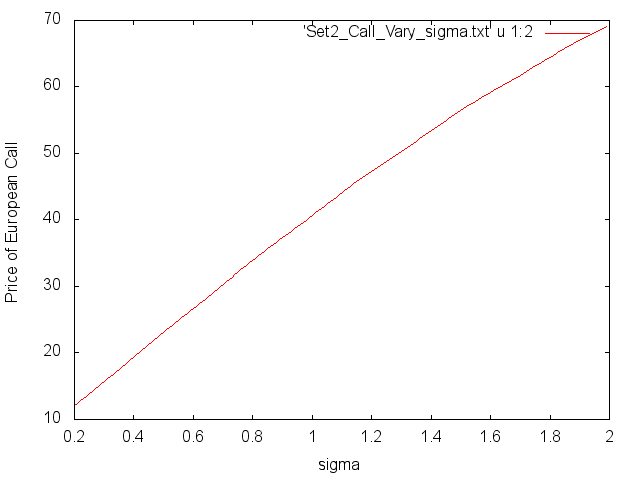
\includegraphics[width =80mm]{Set2_Call_Vary_sigma}\\
(e) Varying M (K = 95) :\\
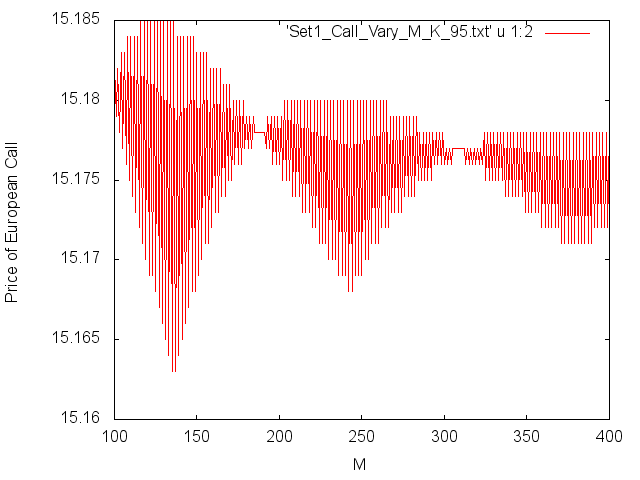
\includegraphics[width =80mm]{Set1_Call_Vary_M_K_95}
\quad \quad
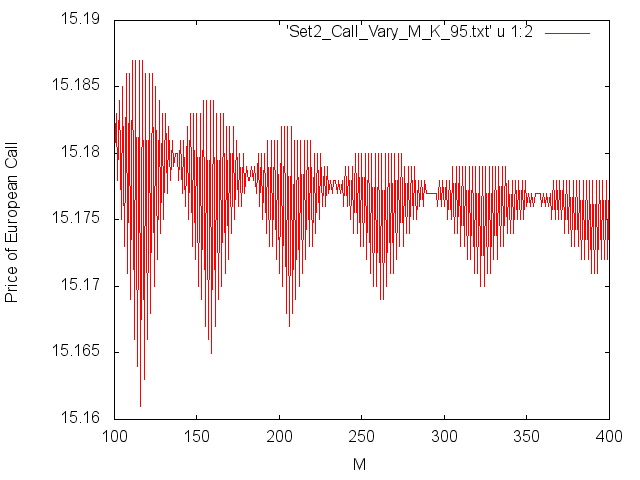
\includegraphics[width =80mm]{Set2_Call_Vary_M_K_95}\\
\newpage
(f) Varying M (K = 100) :\\
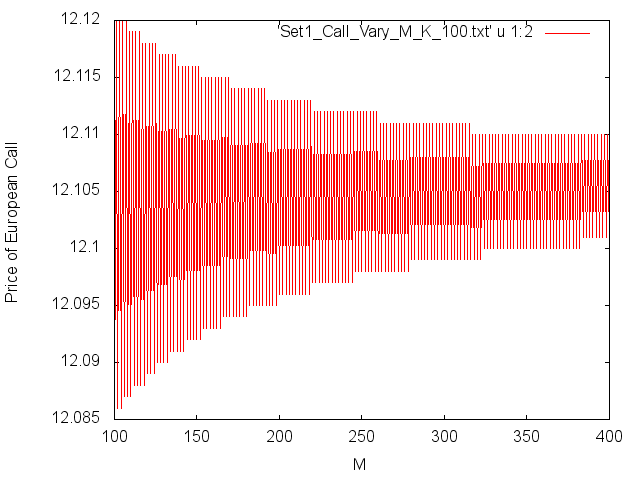
\includegraphics[width =80mm]{Set1_Call_Vary_M_K_100}
\quad \quad
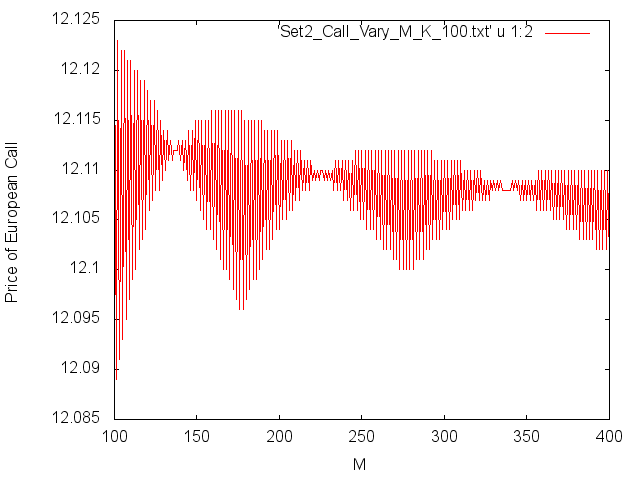
\includegraphics[width =80mm]{Set2_Call_Vary_M_K_100}\\
(g) Varying M (K = 105) :\\
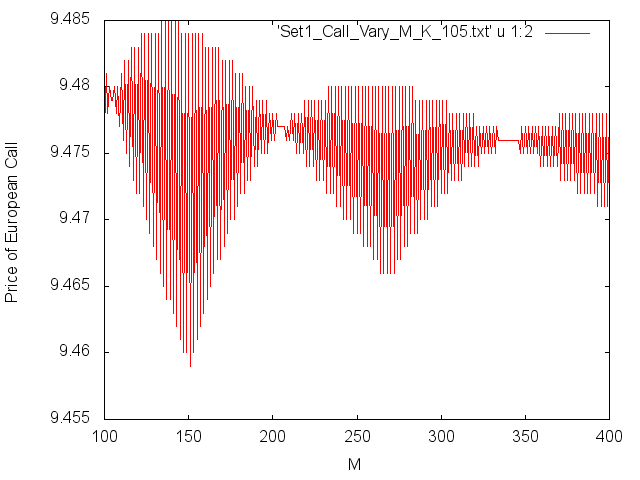
\includegraphics[width =80mm]{Set1_Call_Vary_M_K_105}
\quad \quad
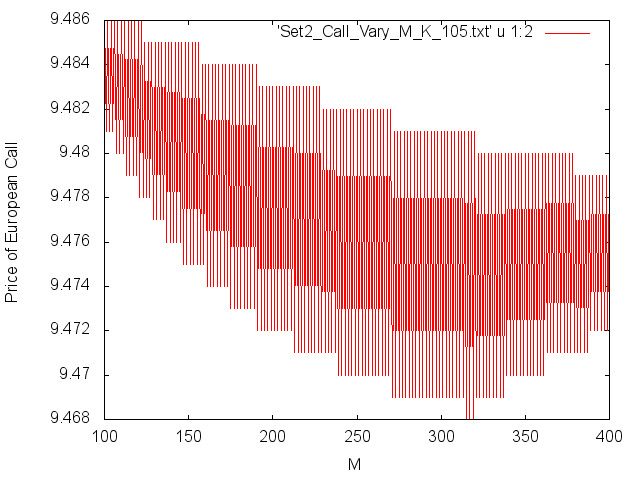
\includegraphics[width =80mm]{Set2_Call_Vary_M_K_105}\\\\

\textbf{European Put Option}\\
(a) Varying S(0) :\\
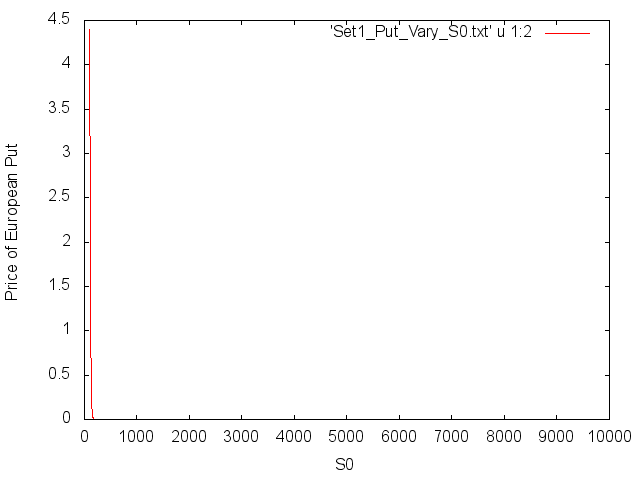
\includegraphics[width =80mm]{Set1_Put_Vary_S0}
\quad \quad
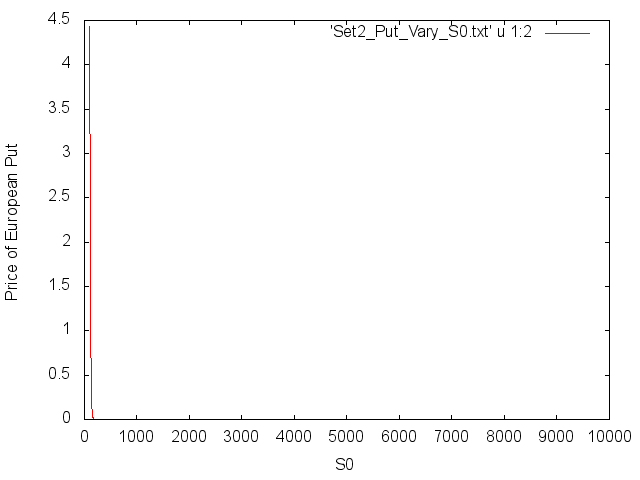
\includegraphics[width =80mm]{Set2_Put_Vary_S0}\\
\newpage
(b) Varying K :\\
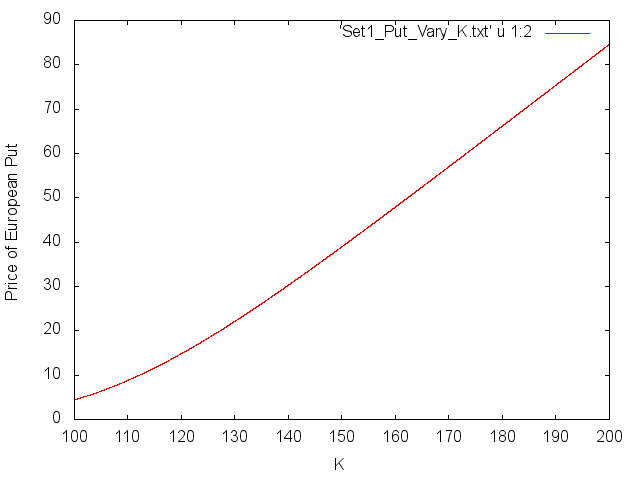
\includegraphics[width =80mm]{Set1_Put_Vary_K}
\quad \quad
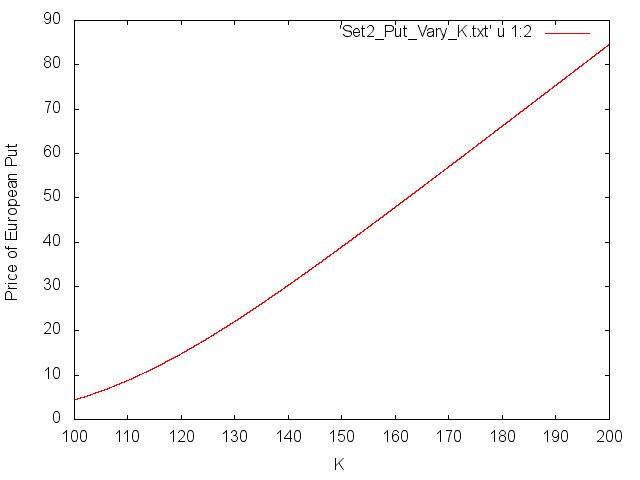
\includegraphics[width =80mm]{Set2_Put_Vary_K}\\
(c) Varying r :\\
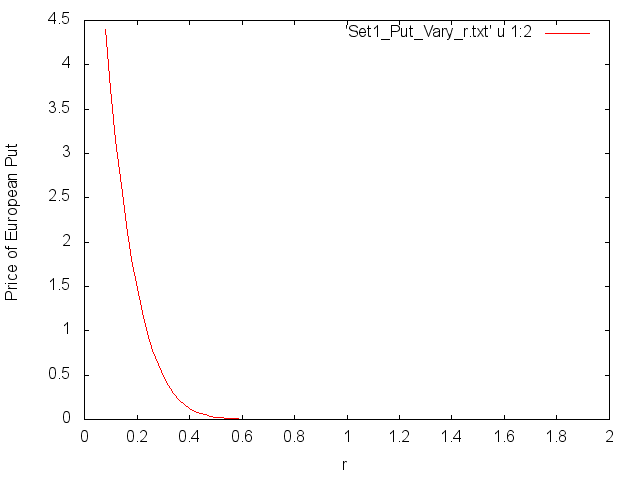
\includegraphics[width =80mm]{Set1_Put_Vary_r}
\quad \quad
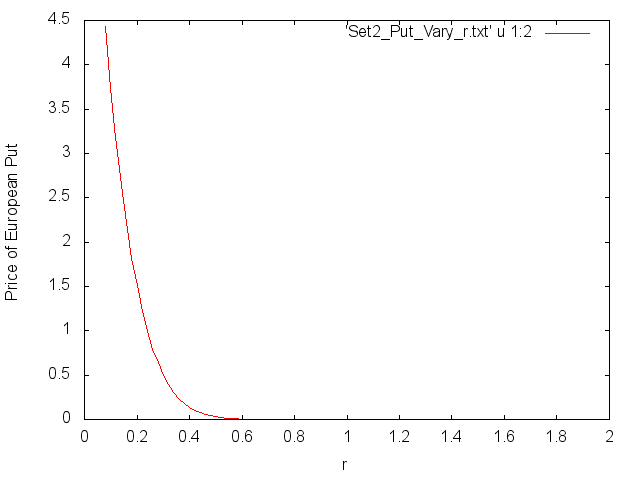
\includegraphics[width =80mm]{Set2_Put_Vary_r}\\
(d) Varying $\sigma$ :\\
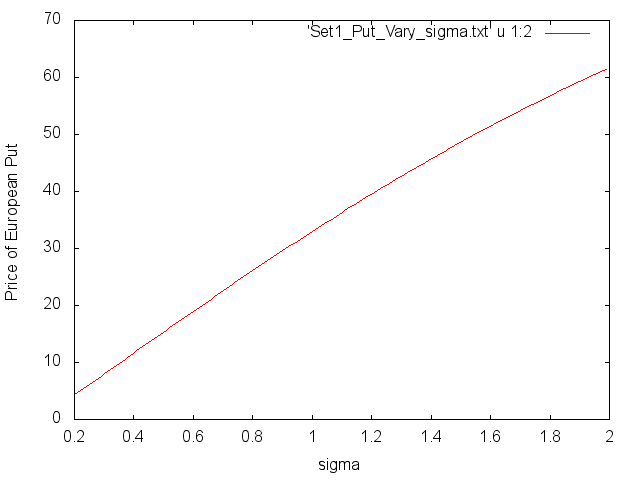
\includegraphics[width =80mm]{Set1_Put_Vary_sigma}
\quad \quad
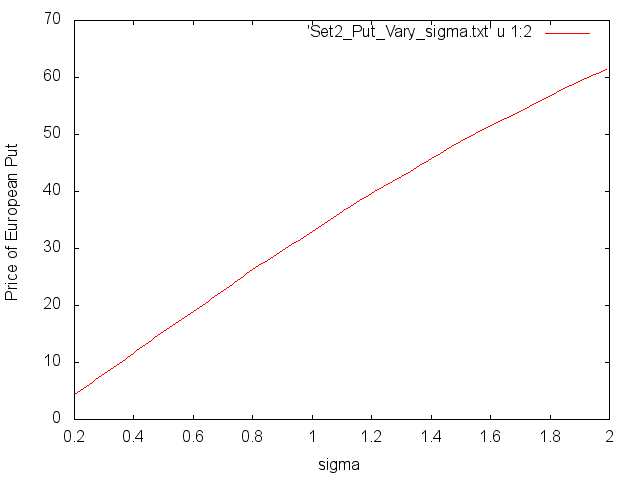
\includegraphics[width =80mm]{Set2_Put_Vary_sigma}\\
\newpage
(e) Varying M (K = 95) :\\
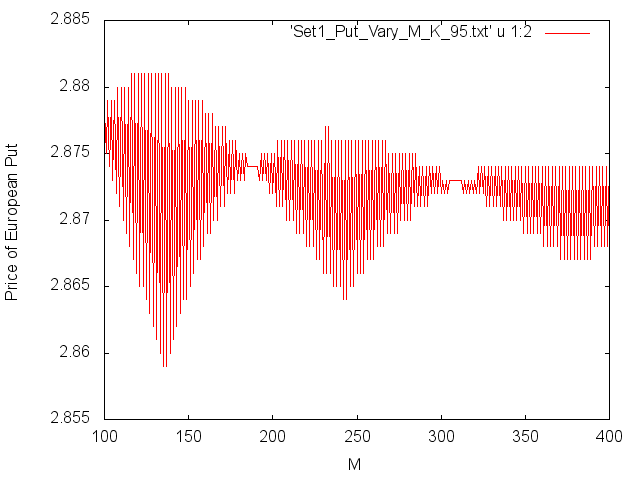
\includegraphics[width =80mm]{Set1_Put_Vary_M_K_95}
\quad \quad
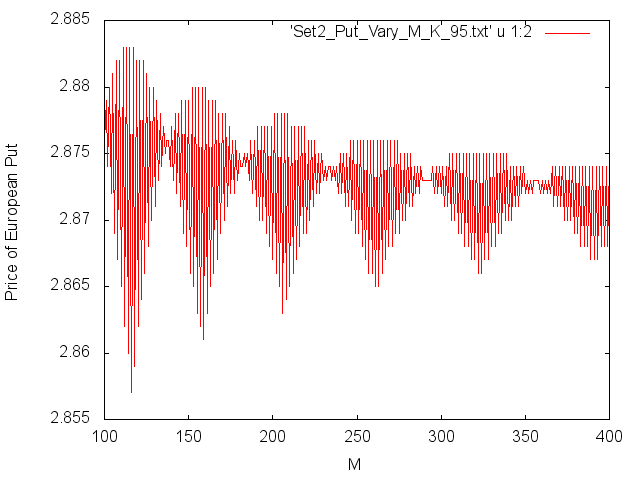
\includegraphics[width =80mm]{Set2_Put_Vary_M_K_95}\\
(f) Varying M (K = 100) :\\
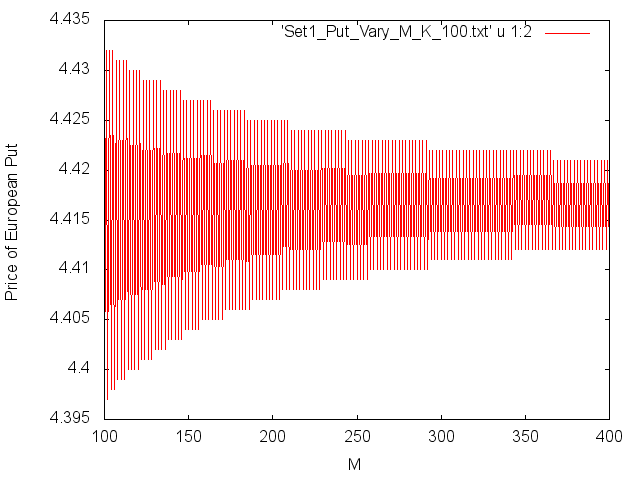
\includegraphics[width =80mm]{Set1_Put_Vary_M_K_100}
\quad \quad
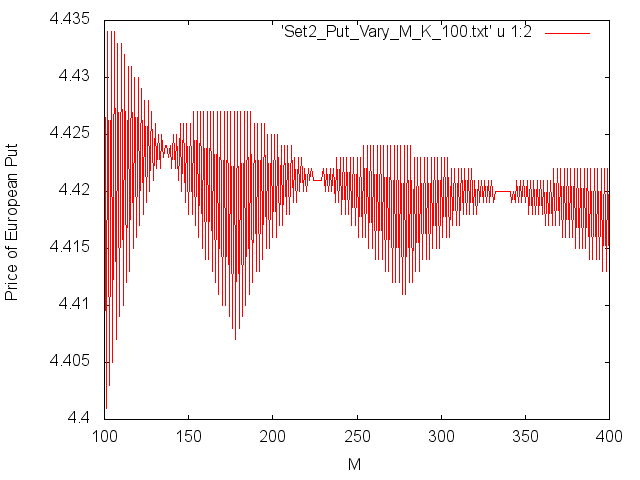
\includegraphics[width =80mm]{Set2_Put_Vary_M_K_100}\\
(g) Varying M (K = 105) :\\
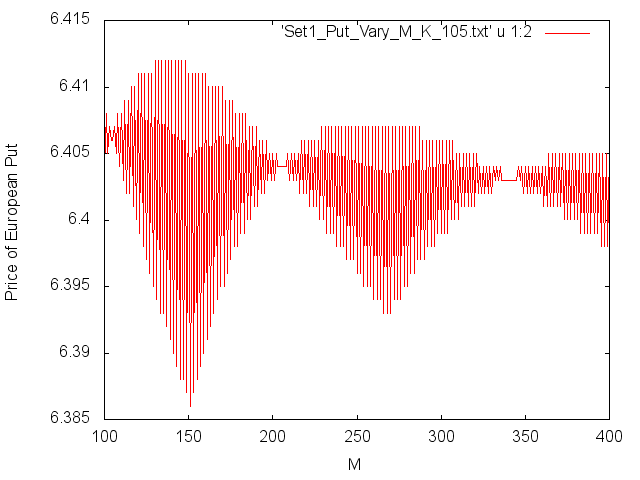
\includegraphics[width =80mm]{Set1_Put_Vary_M_K_105}
\quad \quad
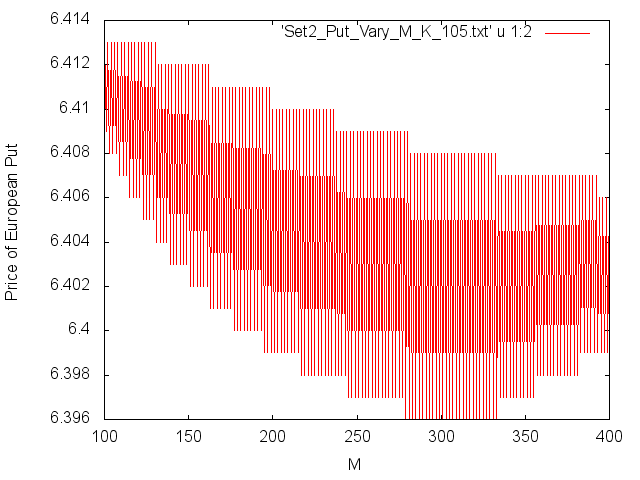
\includegraphics[width =80mm]{Set2_Put_Vary_M_K_105}


\textbf{Observation and Explanation}\\
(1) With increase in S(0), the price of European Call Option increases while price of put decreases. Analyzing with respect to the person long the call , increase in S(0) leads to increase in the market value of stock at maturity hence an increase in the potential payoff from the call option . This leads to an increase in the value/price of the European Call Option. An analogous argument can be given for put option as well.\\
(2) With increase in K ,the price of European Call Option decreases while price of put increases. Analyzing with respect to the person long the call, increase in K leads to lesser payoff, hence the price of call decreases. An analogous argument can be given for put option as well.\\\\
(3) With increase in r, the price of European call option increases while price of put option decreases. Again analyzing with respect to the person long the call ,let's assume the person has S(0) at time t = 0, then the value of S(0) due to risk free rate will be more at maturity now, hence his/her gain is likely to increase, so the price of European Call Option should increase . An analogous argument can be given for put option as well.\\\\
(4) Increase in $\sigma$ has a similar effect as increase in S(0). Increase in M is an oscillatory function of the prices of both the call and put option.

\begin{center}
\textbf{PROBLEM 2}
\end{center}

Now take any path-dependent derivative of your choice and do the above exercise for at least one set (of u , d).

\begin{center}
\textbf{SOLUTION}
\end{center}

\textbf{American Call Option}\\
(a) Varying S(0) :
\begin{center}
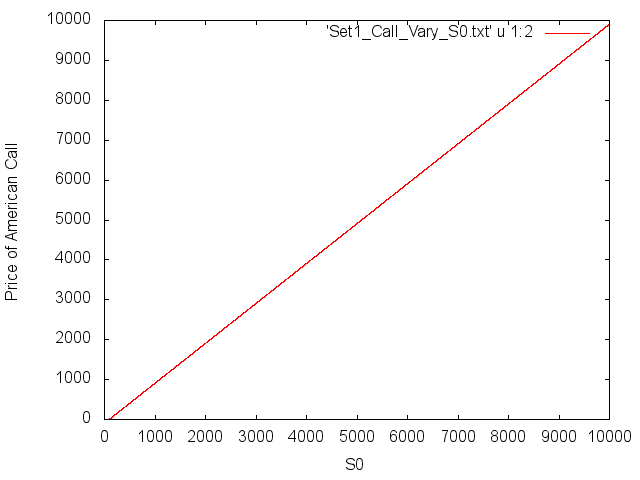
\includegraphics[width =80mm]{Set1_American_Call_Vary_S0}
\end{center}

(b) Varying K :
\begin{center}
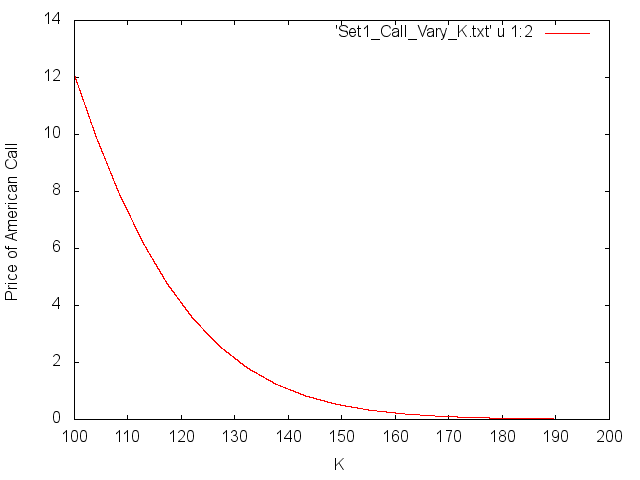
\includegraphics[width =80mm]{Set1_American_Call_Vary_K}\\
\end{center}

(c) Varying r :
\begin{center}
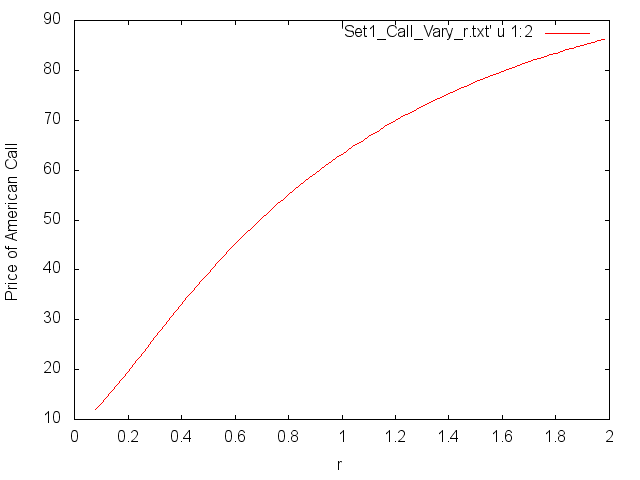
\includegraphics[width =80mm]{Set1_American_Call_Vary_r}
\end{center}

(d) Varying $\sigma$ :
\begin{center}
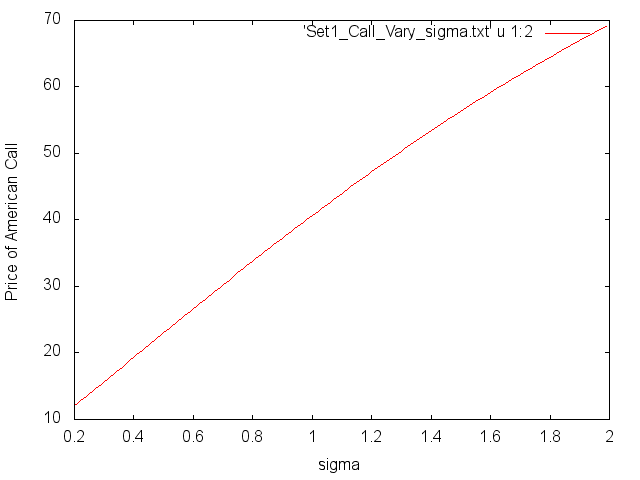
\includegraphics[width =80mm]{Set1_American_Call_Vary_sigma}\\
\end{center}

(e) Varying M (K = 95) :
\begin{center}
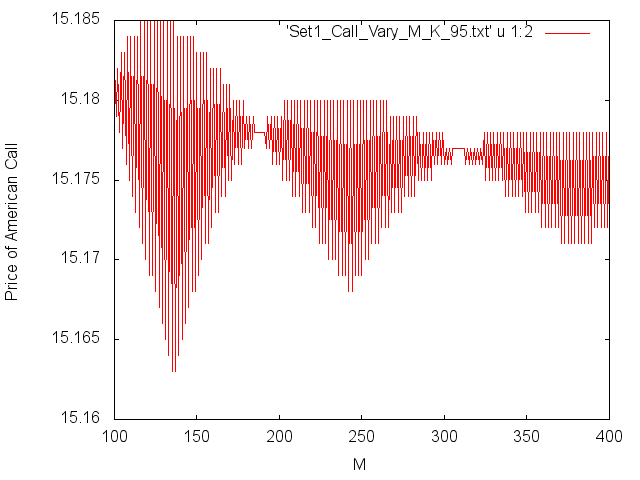
\includegraphics[width =80mm]{Set1_American_Call_Vary_M_K_95}
\end{center}
\newpage
(f) Varying M (K = 100) :
\begin{center}
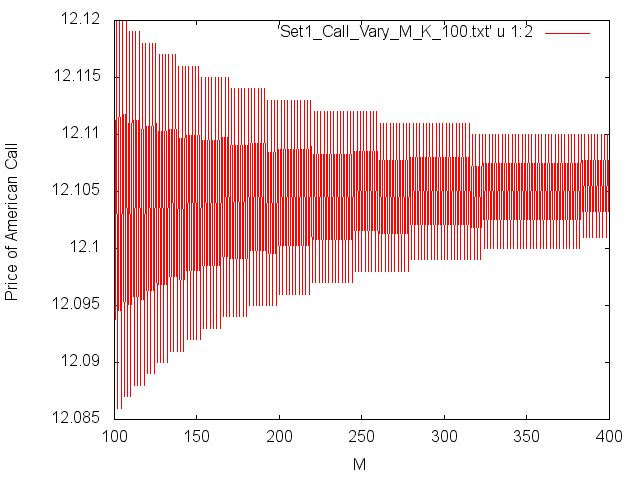
\includegraphics[width =80mm]{Set1_American_Call_Vary_M_K_100}\\
\end{center}

(g) Varying M (K = 105) :
\begin{center}
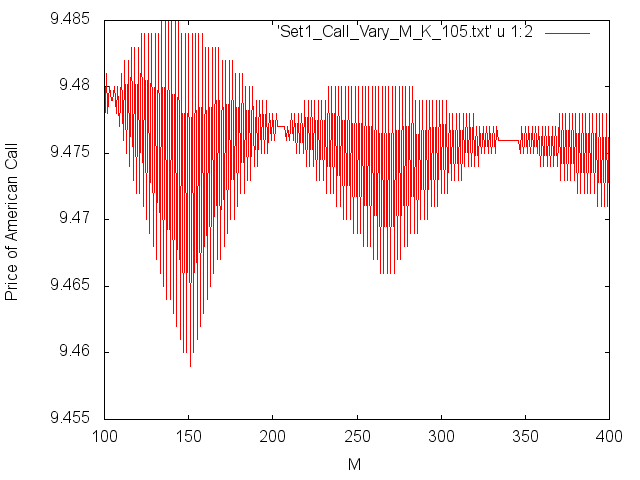
\includegraphics[width =80mm]{Set1_American_Call_Vary_M_K_105}\\
\end{center}

\textbf{American Put Option}\\
(a) Varying S(0) :
\begin{center}
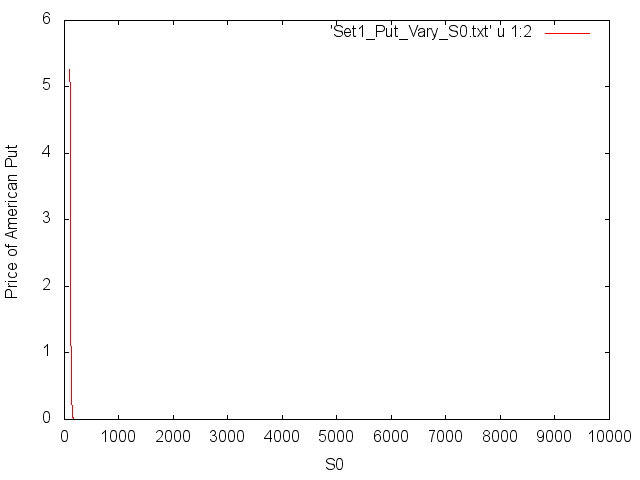
\includegraphics[width =80mm]{Set1_American_Put_Vary_S0}
\end{center}
\newpage
(b) Varying K :
\begin{center}
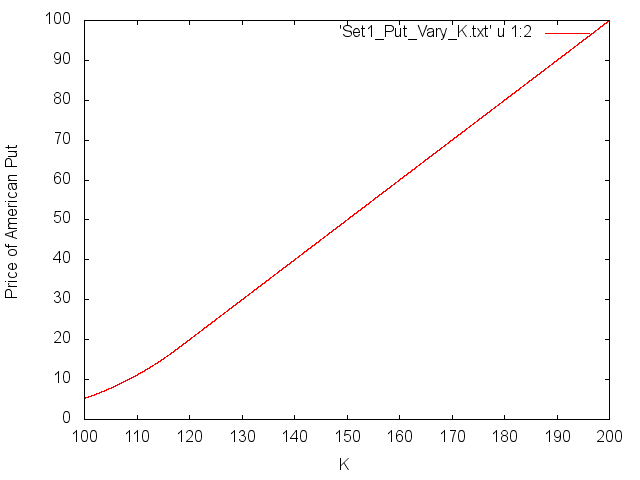
\includegraphics[width =80mm]{Set1_American_Put_Vary_K}\\
\end{center}

(c) Varying r :
\begin{center}
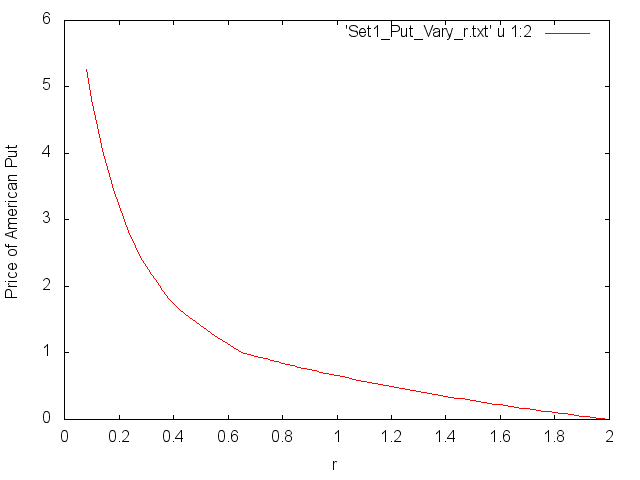
\includegraphics[width =80mm]{Set1_American_Put_Vary_r}
\end{center}

(d) Varying $\sigma$ :
\begin{center}
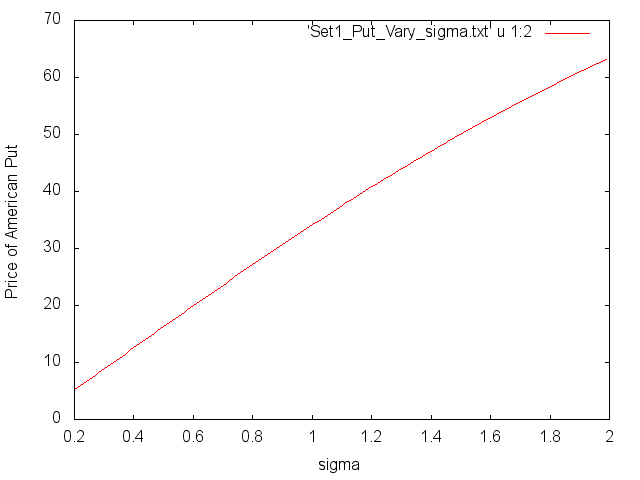
\includegraphics[width =80mm]{Set1_American_Put_Vary_sigma}\\
\end{center}
\newpage
(e) Varying M (K = 95) :
\begin{center}
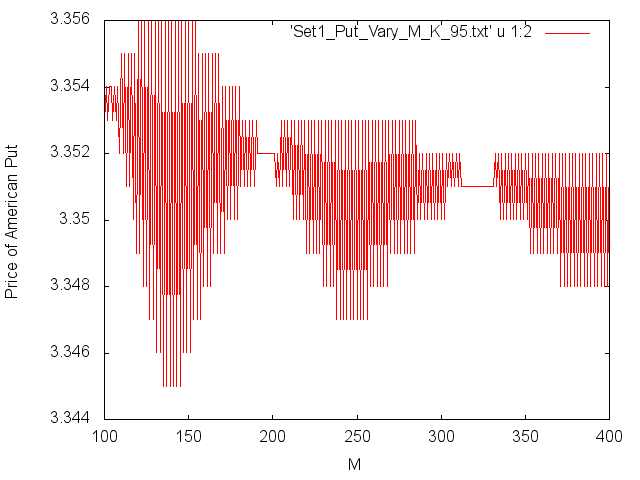
\includegraphics[width =80mm]{Set1_American_Put_Vary_M_K_95}
\end{center}

(f) Varying M (K = 100) :
\begin{center}
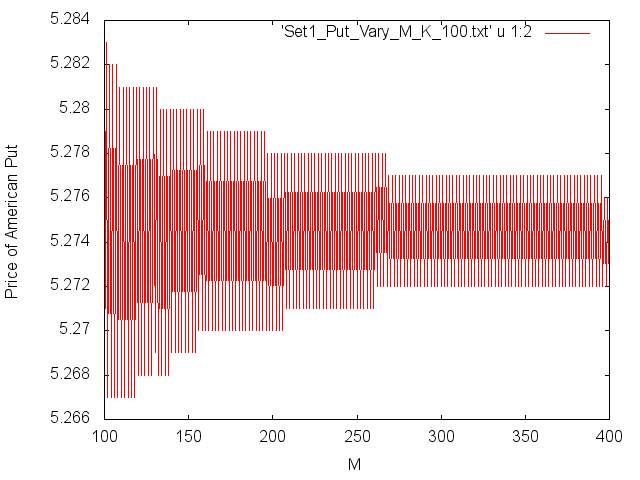
\includegraphics[width =80mm]{Set1_American_Put_Vary_M_K_100}\\
\end{center}

(g) Varying M (K = 105) :
\begin{center}
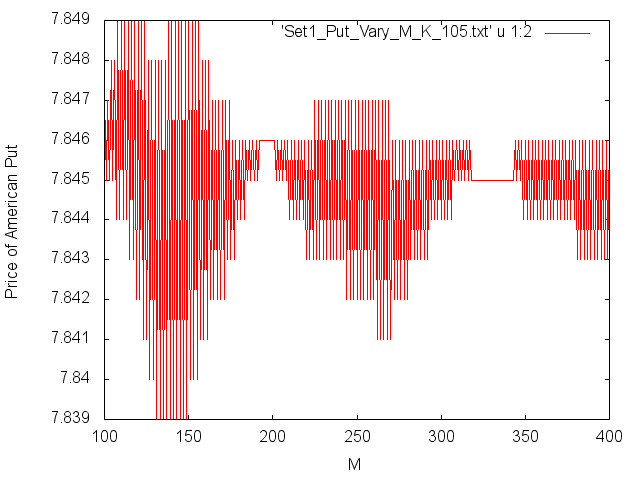
\includegraphics[width =80mm]{Set1_American_Put_Vary_M_K_105}
\end{center}
\newpage
\textbf{Observation and Explanation}\\
(1) The path dependent option taken is the American option which can be accessed at any instant of time. The value of the option is the maximum out of the risk-neutral value and the intrinsic value. The set chosen for u and d is Set - 1.\\\\
(2) The variation is similar to that of European Call and Put option, and the reason behind the trends are also similar. The only difference here is the access time which is not fixed.
\end{document}